\cleardoublepage
\chapter[Band structures of semiconductors and insulators]{Band structures of semiconductors\break and insulators\label{ch:band-structures}}
In this chapter we discuss the details of practical calculations, and the results obtained for a manifold of reference insulating materials. Thanks to the validity of Bloch's theorem, discussed in \cref{ch:koopmans-periodic}, it is possible to obtain electronic band structures -- within the primitive cell's BZ -- either from a supercell approach, by means of an unfolding method, or from the primitive cell implementation described in \cref{sec:koopmans-pbc}. The computational details of the calculations, including the description of the unfolding method and of the Koopmans workflow, are discussed in \cref{sec:calculations-koopmans}, while in \cref{sec:results-bands} we report the obtained results.

Part of the content of this chapter, as well as the reported results, have been published in Refs.~\cite{de_gennaro_blochs_2022,colonna_koopmans_2022}.

\clearpage
\section{Calculations with Koopmans functionals\label{sec:calculations-koopmans}}
Electronic-structure calculations using Koopmans spectral functionals are performed following two different approaches, based on the two strategies to compute the screening parameters discussed in \cref{sec:screening-parameters}: the first makes use of the finite energy differences strategy and relies on the SC method, the second resorts to linear response theory and takes full advantage of the system's symmetries by exploiting the Wannier-like nature of the variational orbitals.

The former represents the original approach used to perform the first calculations in crystalline materials \cite{nguyen_koopmans-compliant_2018}, although, in that case, the quasiparticle energies were computed only at the $\Gamma$-point of the SC (no information about the $\bk$-dispersion). By means of an unfolding technique -- which, once again seizes on the fact that the variational orbitals are WFs, to reconstruct the $\bk$-dependence of the Koopmans Hamiltonian -- here we show, for the very first time, band structures calculations from Koopmans functionals along any path in the BZ \cite{de_gennaro_blochs_2022}. From now on, when speaking of the BZ, we will implicitly refer to the PC's BZ, since the one of the SC always consists of the $\Gamma$-point only.

The second approach came out more recently \cite{colonna_koopmans_2022} and, since it relies on a second-order approximation of the $\Pi_i$ terms, so far it has been developed only for the KI functional. Differently from the SC approach, it does not compute the ground state in a variational way, but rather opts for the very reasonable 

A big part of this thesis was dedicated to the development of some parts of the computational code, to reach a stable implementation working for periodic systems, together with an optimization of the entire workflow required to perform calculations of Koopmans functionals in crystalline materials. In the following sections we give a detailed description of these aspects.


\subsection{Unfolding method\label{sec:unfolding-method}}

\begin{figure}
    \centering
    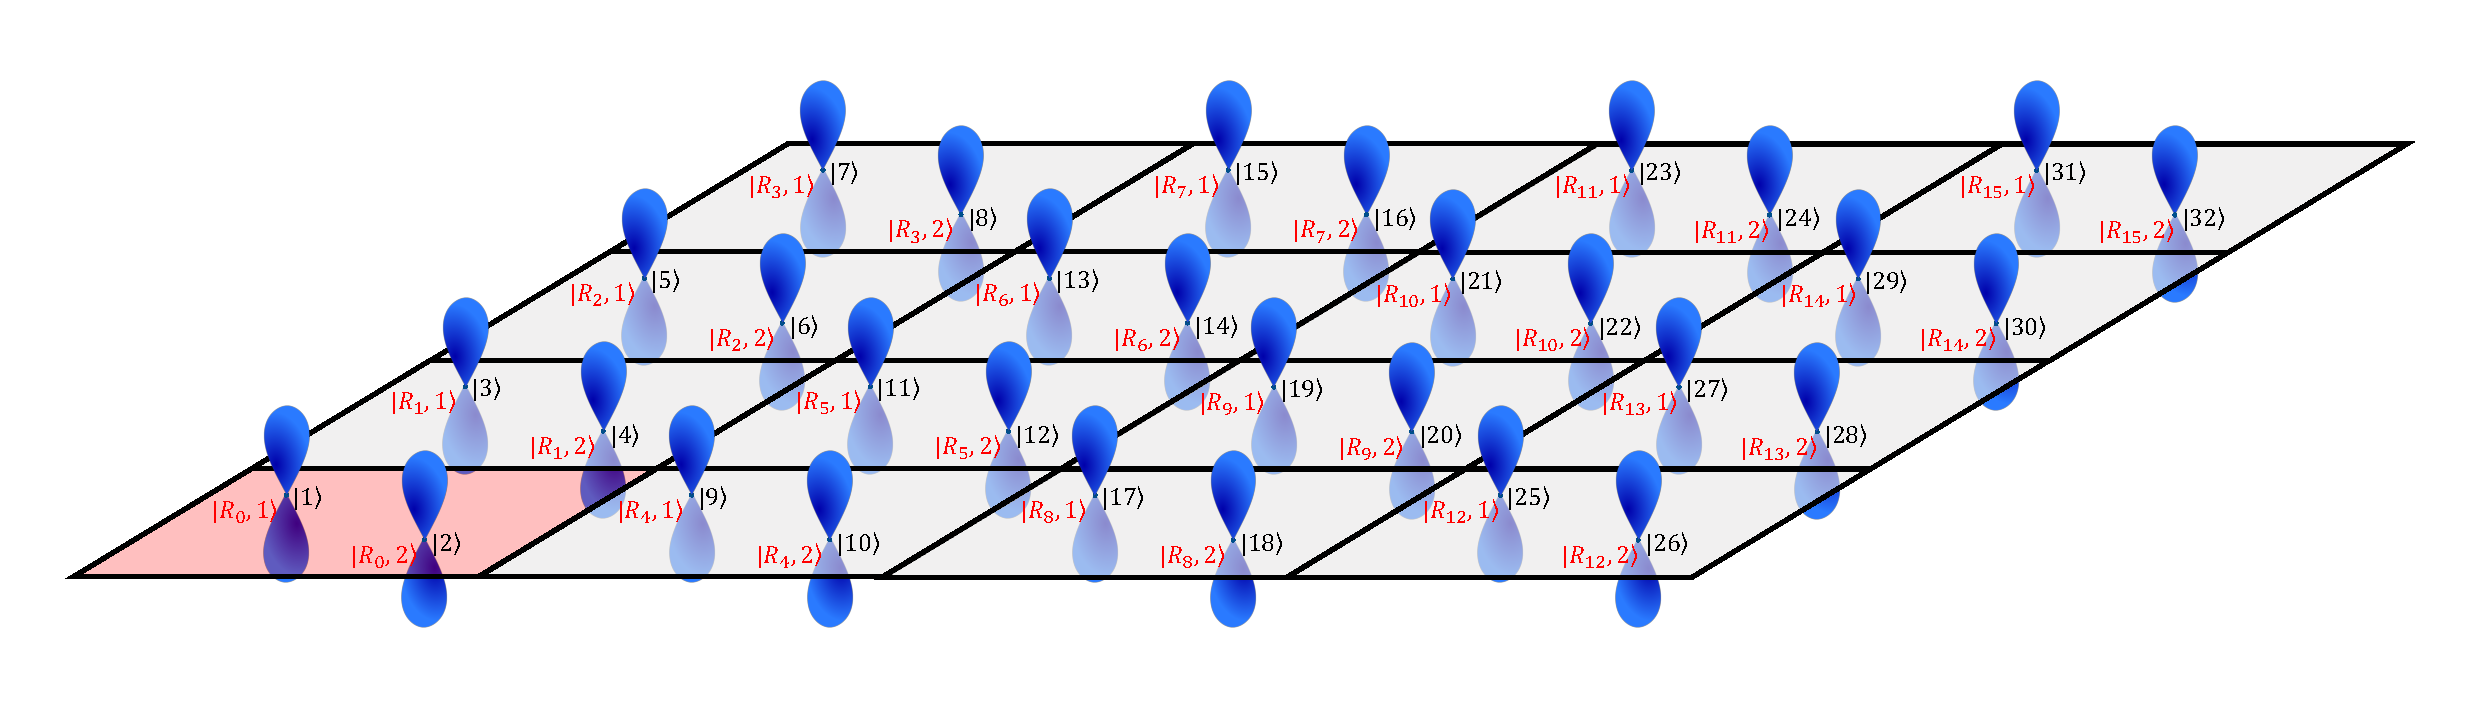
\includegraphics[width=\linewidth]{WF-pcell-scell.pdf}
    \caption[]{}
    \label{fig:map-wf}
\end{figure}


\subsection{Workflow\label{sec:workflow}}

\begin{figure}
    \centering
    \subfloat[]{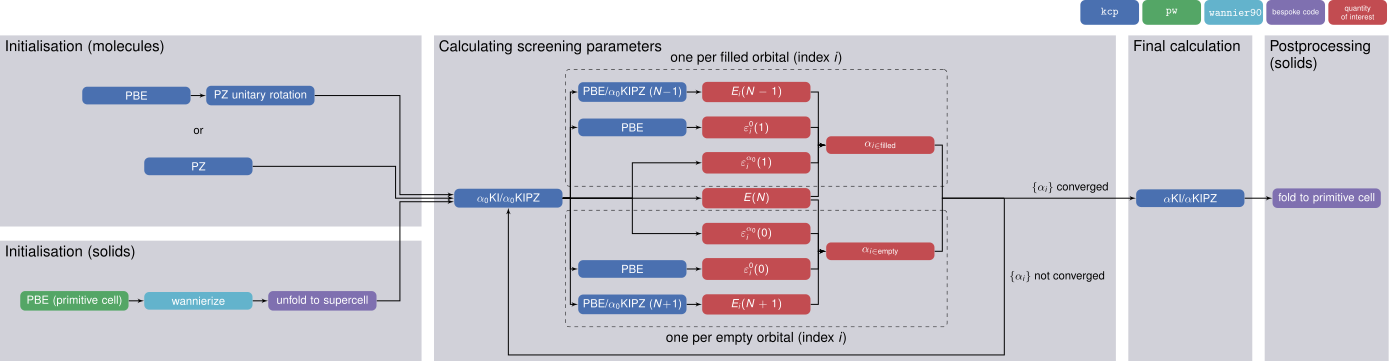
\includegraphics[width=\linewidth]{dscf_workflow.png}} \\
    \subfloat[]{
\includegraphics[width=\linewidth]{dfpt_workflow.png}}
    \caption[]{}
    \label{fig:workflow}
\end{figure}

\subsection{Computational details\label{sec:computational-details}}

\section{Results\label{sec:results-bands}}

\subsection{Finite differences\label{sec:results-dscf}}

\subsection{DFPT\label{sec:results-dfpt}}

